\chapter{Research Methodology}
\label{ch:Methodology}
This chapter introduces the research methodology selected in this project, including both high-level design and low-level tool for implementation.
\section{Problem Definition}

The main task of this project is to find an appropriate method to group stock market data. In this project, the stock market data are defined as $X = (X_1, \cdots, X_N) \in \mathbb{R}^{N \times T \times D} $, where $X_m = (x_{m_1},\cdots, x_{m_T}) \in \mathbb{R}^{T \times D} $ represents all historical series of a single stock, N is the number of stocks, T is the number of time slices, D is the dimension of a single data. This task is further divided into 4 sub-tasks: (1) time-series data preprocessing; (2) time-series data transformation; (3) time-series data clustering; (4) experiments and evaluation.

\section{Guideline for this project}
\label{sec:invariance}
This project aims to group stocks by their annual trends, however, according to \cite{batista2014cid}, sequences data are often distorted in some way in different domain, directly compare distorted sequences could be meaningless. To make the clustering results more informative, make the general trend more representative, this project follows a sequence comparison guideline. The guideline chosen here inherits from the known time-series invariances summarized by \cite{paparrizos2015k}. This project follows it to process stock data, find an appropriate method to group stock data and choose an appropriate metric to evaluate the clustering results. Followings are the details of the guideline.
\begin{enumerate}
    \item Scaling and offset invariance: due to the different amplitudes (or scaling) and offset (or translation), two sequences may not match well despite they have similar shape and trend. For example, given a sequence $\vec{x}$ and its variation $\vec{x\prime} = a\vec{x} + b$, where a and b are constants, their similarity to other sequences should be the same. This property is important especially for the comparison of two stocks with different price range and hence is required. Figure~\ref{fig:scalinv} shows an example of scaling and offset invariance, in these two subfigures, blue lines are the same, while red lines have different scaling. Both the red lines should be treated similar to the blue line, however, directly applying distance measure to the bottom example may not able to reflect that.
    \begin{figure}[!htbp]
        \centering 
        \subfigure[] { \label{fig:scaleinv1} 
        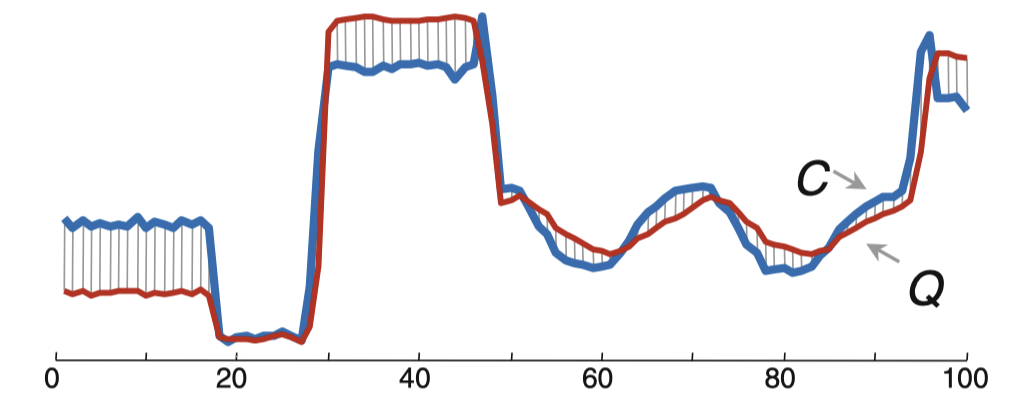
\includegraphics[width=0.4\columnwidth]{scaleinv1.png} 
        } 

        \subfigure[] { \label{fig:scaleinv2} 
        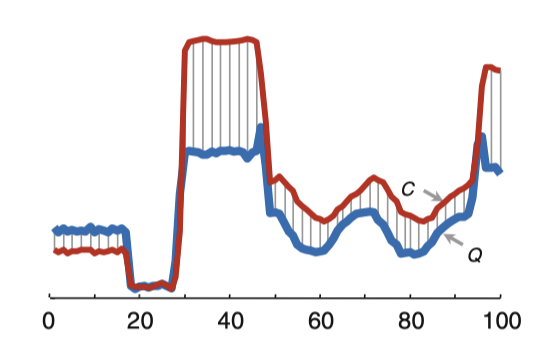
\includegraphics[width=0.4\columnwidth]{scaleinv2.png} 
        } 
        \caption{Example of scaling and offset invariance (Source:\cite{batista2014cid})} 
        \label{fig:scalinv} 
    \end{figure} 
    \item Local scaling invariance: given two sequences with same length, if they are aligned globally or locally, they should be considered as a similar pair. The term ``global alignment'' means the general trend of the two sequences are similar but differ in some subsequences. To the contrary, ``local alignment'' means there are some regions of two sequences match well while other parts do not. Such invariance is crucial for some trajectories with different speed (such as the movement of different people). Figure~\ref{fig:localinv} shows an example of such invariances, these two sequences are regarded as similar. In terms of stock sequences, such invariance can help to group stocks with similar trend but different trend duration together and hence is required.
    \begin{figure}[!htbp]
        \centering
        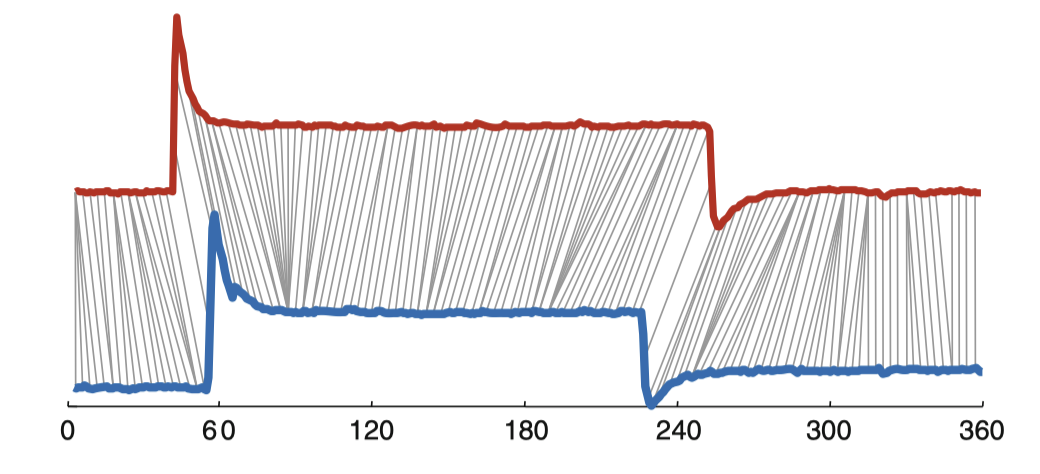
\includegraphics[width=0.5 \columnwidth]{localinv.png}
        \caption{Example of local scaling invariance (Source:\cite{batista2014cid})}
        \label{fig:localinv}
    \end{figure} 
    \item Global scaling invariance: different from local scaling invariance, global scaling invariance is about length-varying sequences. If two sequences have a similar shape but different length, they should also be grouped together. Figure~\ref{fig:globalinv} shows an example of global scaling invariance, CDC is a full gene expression and it matches poorly to the prefix of a related gene sequence, CDC15. However, if it is rescaled by a factor of 1.41, it can matches CDC15 more closely. In terms of stock sequences, due to numerous factors, the length of each records can be different, hence such invariance should be considered.
    \begin{figure}[!htbp]
        \centering
        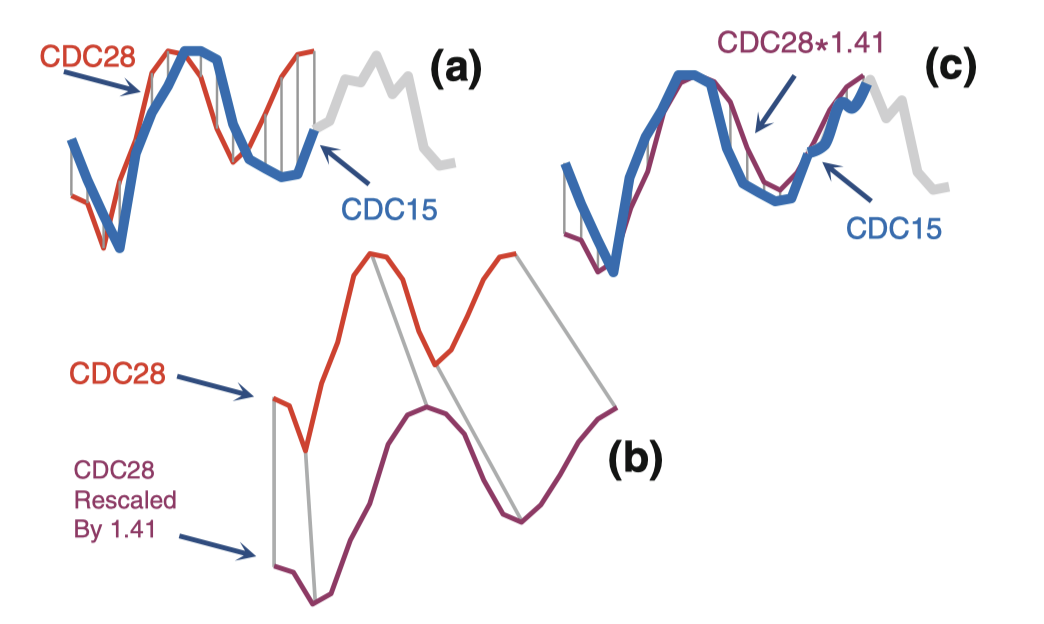
\includegraphics[width=0.5 \columnwidth]{globalinv.png}
        \caption{Example of global scaling invariance (Source:\cite{batista2014cid})}
        \label{fig:globalinv}
    \end{figure} 
    \item Complexity invariance: if two sequences have similar shape but different frequencies (complexity), they should be grouped together. This invariance is crucial for stock prices analysis, since the stock sequences contains massive short term small fluctuations that do not change the general shape but affect the comparison of stocks.
\end{enumerate}
Those invariances are basic standards of how this project measures the similarity of two stocks. Following sections explain how to apply them in programming and experiments.

\section{Stock Data Preprocessing}
\label{sec:Preprocessing}
According to \cite{paparrizos2015k}, scaling and offset invariance and complexity invariance can be achieved by data processing while other invariances can not. Therefore, this project adds a data preprocessing phase before futher analysis. The main steps include:
\begin{enumerate}
    \item Data denoising: this step is highly associated with complexity invariance. According to the guideline, the small fluctuations on stocks should not impair the similarity measure. Commonly used distance measures such as Euclidean distance and Cosin distance can not deal with such fluctuations. This project uses data denoising (or called data smoothing) to alleviate the issue. The detailed method and its effect can be seen in Section~\ref{sec:denosing}
    \item Data normalization: this step is highly associated with scaling and offset invariance. After normalization, sequence $\vec{x\prime} = a\vec{x} + b$ will be treated as the same with sequence $x$. Theoretically, both Z-Score and Min-Max normalization can achieve this, and their effect and comparison can be seen in Section~\ref{sec:normalization}
\end{enumerate}
Note that based on the guideline, the final experiments and visualization are conducted on the pre-processed data rather than the raw data. For those invariances that can not be achieved by simple processing methods, this project seeks help from data representation algorithm and evaluation metrics.

\section{Stock Data Representation}
\label{sec:Feature}
Feature engineering attempts to find the latent features of original data that can improve the performance of machine learning algorithms. By research, there are various traditional and novel representation algorithms for time-series data, each of them achieves certain invariances. This project tries to apply them to this project to test whether they are suitable for trend-based time-series clustering tasks. The introduction of different representations can be found in Chapter \ref{cha:representation}.

\section{Stock Data Clustering}
In this project, the representative trends of stocks are produced by clustering algorithms. Different from other works that mainly test the performance of various clustering algorithms with the original sequences, our interest is that whether those traditional and novel representations with a simple cluster algorithm can produce a good result. Hence this project mainly uses one clustering algorithm KMeans. To get more universal observations ans conclusions, this project may use other clustering algorithms, but not in all experiments.



\section{Evaluation}
\label{sec:Evaluation}
The evaluation of this project is conducted on each phase. This decision benefits the ablation study. For different phase, there could be different metrics and criteria, but in generally, they follow the above guideline. In preprocessing phase, both visual and numerical comparison are used to evaluate different methods since their effects are easy to understand. In representation phase, mainly the visual comparison is used, since there is no direct metric to compare different representation algorithms. The numerical comparison of different representations hence is conducted in the clustering phase. In clustering phase, both visual and numerical comparison are used, since the data doesn't have labels, indexes that does not require ground truth information are chosen as the metrics.

\section{Tools for Implementation}
This project is developed by Python programming language, since there are various out-of-box libraries for data analysis. The main libraries used to build this project include: Numpy, Matplotlib, Scikit-learn, Tslearn, Seglearn, Pyts, Pywt and Pytorch. Numpy provides the basic operations for manipulating vectors and matrixes. Matplotlib provides numerous functions to display the data and the experimental results. Scikit-learn provides well-optimized implementation of basic machine learning algorithms, including the clustering algorithms such as KMeans, DBSCAN and some evaluation metrics. Tslearn, Seglearn and Pyts are libraries for time-series data preprocessing, they provide functions such as segmenting data, scaling the data and extracting statistical features. Pywt provides various sequence decomposition methods, and it is used to denoise the data. Pytorch provide functions to build, train and store ANNs, it can use GPU to boost the computation. Other functions are purely implemented by Python.

\section{Chapter Summary}
This chapter introduces the research methodology of this project. The basic research guideline is proposed based on the invariances of stock market data. This guideline indicates what kind of stock price sequences should be treated as similar. Then, according to the guideline, the preprocessing steps, representation methods, clustering algorithms and the evaluation metrics are discussed and selected. Finally, implementation tools of this project are introduced.